\section{公共卫生体系下的治未病}
\subsection{治未病政策发展}
\subsubsection{试点阶段}
2007年至2015年,国家中医药管理局开展“治未病”健康工程以后,全国先后确立了 65 个地区开展“治未病”预防保健服务试点,4 批共 173 家“治未病”预防保健服务试点单位,试点范围由中医医院逐步扩大到综合医院、专科医院、社区卫生服务机构以及中医药预防保健服务专门机构,建立了“治未病中心”服务点。试点单位使用昆仑——炎黄公司开发的“中医健康保障服务模式”,形成了体质辨识门诊、健康调养咨询门诊及传统疗法中心“三位一体”的运作模式。同时鼓励社会力量投资兴办中医预防保健服务机构。
\subsubsection{“慢病”落实阶段}
2012 年原卫生部等15 部委联合印发了《中国慢性病防治工作规划(2012—2015)》,2014 年卫生部出台《中国居民慢性病与营养监测工作方案》,将“治未病”理念落实到慢病这一具体疾病类型,把原来的治疗转化为规范性的预防、筛查、检测、治疗。同时这一阶段进行的分级诊疗制度建设创新了治未病的形式,建立基层签约服务制度。

通过政策引导,推进居民或家庭自愿与签约医生团队签订服务协议。签约医生团队由二级以上医院医师与基层医疗卫生机构的医务人员组成,通过定时上门体检与电话回访来实时预防检测慢病的产生治疗。由于这一制度属于预防与治疗的结合,因此,这一签约制度同时也加强了慢病未病先防观念的普及。这一政策的意义还在于将治未病这一理念与客观存在的病相结合,在行动上做到有的放矢。
2017年国务院发布的国民营养计划(2017—2030年)将未病先防观念落实到生活的各方面。
\subsubsection{互联网+阶段}
2015 年国务院出台《关于积极推进“互联网 +”行动的指导意见》,提出发展基于互联网的医疗卫生服务,探索电子处方等网络医疗健康服务应用,同年的 12 月,乌镇互联网医院开出了第一张电子处方。在宏观政策层面,国家支持并鼓励建立医疗数据搭建信息化平台,互联网医疗企业利用自身技术优势搭建信息共享平台,有利于整合疾病信息,连续、及时地监测数据,方便就医时获得准确、有效的医疗服务,尤其是慢病患者的电子档案。传统的中医宣传方式如国家中医药管理局开展的中医角与中医文化知识竞赛已不能满足当前的宣传科普需要。

\begin{spacing}{1.19}
\begin{table}[]
    \centering
    \begin{tabular}{|c|c|c|}
        \hline
        \rowcolor[HTML]{FFFFFF} 
        文件名称                          & 颁布单位     & 年份   \\ \hline
        \rowcolor[HTML]{FFFFFF} 
        “十三五”深化医药卫生体制改革规划             & 国务院      & 2016 \\ \hline
        \rowcolor[HTML]{FFFFFF} 
        “十三五”国家科技创新规划                 & 国务院      & 2016 \\ \hline
        中医药发展战略规划纲要(2016—2030年)       & 国务院      & 2016 \\ \hline
        中国防治慢性中长期规划(2017—2025年)       & 国务院      & 2017 \\ \hline
        国务院办公厅关于支持社会力量提供多层次多样化医疗服务的意见 & 国务院      & 2017 \\ \hline
        国民营养计划(2017—2030年)            & 国务院      & 2017 \\ \hline
        医疗卫生领域中央与地方财政事权和支出责任划分改革方案    & 国务院      & 2018 \\ \hline
        中医药健康文化知识角建设指南                & 国家中医药管理局 & 2018 \\ \hline
    \end{tabular}
    \caption{2016-2018治未病相关政策}
\end{table}

\end{spacing}
\subsection{社区医院角色}
社区卫生服务中心是公益性、综合性的基层医疗卫生机构,承担着常见病和多发病的诊疗、基本公共卫生服务、计划生育技术服务、健康管理、危急重症病人的初步现场急救和转诊等功能任务,是城乡医疗卫生服务体系的基础。
\subsubsection{与居委会}
社区医院作为整个体系中唯一具有专业医学知识的一环,它可以向居委会输出“治未病”的知识及有关人员。目前宣传“治未病”的方式主要有横幅、知识长廊、讲座等,而社区医院就可以用自己的专业知识以及对“治未病”的理解去撰写“治未病”宣传横幅,撰写介绍“治未病”和如何“治未病”的科普文章,然后交给居委会完成贴横幅,贴科普文章等宣传工作,也可以对居委会人员进行“治未病”培训,让居委会直接在与居民交谈过程中向居民传播“治未病”相关知识。

同样的,居委会可以为一场讲座提供场地、后勤人员,并宣传讲座内容,组织居民报名,而社区医院可以为一场讲座提供讲师,实现形式有社区医院内部人员,聘请外部相关人员,以及在居委会中培训出有能力的人员。
\subsubsection{与居民}
社区医院最主要的职能为向居民提供医疗服务,而在治未病体系中,社区医院可以直接的向上门看病的居民提供“治未病”知识,例如门诊交谈时向居民传播“治未病”相关思想以及“治未病”与居民病症的联系,在医院门口放置“治未病”传单供人取阅,以及在医院内部张贴“治未病”宣传海报等。

当然,社区医院也可以让“治未病”融入治疗中:对于前来就诊的患者可以宣传一些养生知识,例如饮食搭配,日常锻炼,养生保健操等。也可以对身体处于亚健康状态的居民使用中药来调理身体,在染上疾病之前就预先采取措施,这也是“治未病”的一种可行有效的方式。
\subsection{居委会角色}
\subsubsection{与社区医院}
居委会作为协助人民政府或者其它的派出机关做好与居民利益有关的公共卫生的机构。居委会通过其掌握的途径与社区医院取得联系,邀请社区医院的专业医疗机构人员走进社区,并作为居民与社区医院的桥梁,开展普及中医养生保健的讲座等,促使居民进一步了解中医养生以及“治未病”的相关内涵。此外,居委会还能将居民的诉求反馈给社区医院,使社区医院更加清晰基层百姓所需要的是为何种医疗关注,更有利于医疗机构进行针对性的医疗健康服务。

\subsubsection{与居民}
居委会为居民的医疗保健活动提供场地,利用其宣传号召的能力,组织启发居民们参与到活动中来。居委会所独具的亲和力与凝聚力使得此类基层医疗健康工作得以更深层、更广泛地开展。而居委会对所管辖的居民进行的随访,则更近距离关注基层卫生情况,关心百姓民众的健康状况。以此亲切的,口耳相传的方式,使得居民更能感受到政策的温度,进一步提高了他们对于参与到“治未病”医疗健康体系中的能动性。

居委会发挥着联系居民与社区医院两方并组织开展预防保健方面的活动,如体检、讲坛等的作用。就联系居民的方式而言,居委会主要通过网格制度和居民取得联系。网格一般指社区按居民楼分布进行的区域性划分。一个社区工作人员分管 5-6 栋居民楼,规模 500 人左右,形成了一个网格。居委会利用网格制度,一方面向居民传递健康方面的信息,另一方面接受居民对社区建设的意见。其中,东方城社区充分利用互联网,建立了 QQ、 微信群等;五福家园社区通过居民骨干,即楼层长制度来充当联系人的角色,亦类似网格所代表的区域划分思路。

此外,居委会也定期组织居民参与到预防保健活动中来,这些活动基于公共卫生管理的考量,其内容有一部分属于中医治未病的范畴。例如,东方城居委会通过立项的方式响应居民需求。在预防保健方面,开设健康讲堂、定期组织职工体检、关心走访慢性病人、同社区医院联动进行义诊等等。可以发现,尽管上述的服务涉及到中医治未病的部分,但是尚未出现专门有以治未病为名义的相关立项。不管是居民还是居委会,他们都表现出对于治未病一词的陌生,但是如果将这一词语的内涵缩小至“预防疾病”这一种,便能得到理解。

\subsection{居民角色}
\subsubsection{与居委会}
居民向居委会反馈基层卫生情况,并向居委会反映医疗诉求。居民在面对居委会时,更能将自身的细节性健康诉求表达出来,因此能更真实反映民众的情况。实地调查后发现,居民通过居委会组建的网格制度,可以通过向楼长以及通过互联网的形式表达自己的诉求及建议。
\subsubsection{与社区医院}
居民为社区医院提供病案的真实反馈,居民在与医生交流过程中将阐述自身的生理病理情况,以便于医生给出专业性的解释。

居民访谈来看,居民遇病才会求医,不会主动寻求保健服务,对于保健知识中 青年也没有过多的追逐热情。对于老年居民,他们有切身的健康诉求,但是往往由于社区医院的服务不够完善而流向大型三甲医院。
由于社区医院资源有限,居民难免会有轻侮的心理,不信任社区医院的服务,导致基层医院对于中青年人的吸引力很小。而对于职工待遇好的老年人,他们则直接和相应的定点医院联动,也不和社区医院有所交集。
\subsection{小结}
最后通过图例说明三者之间的互动和联系。

\begin{figure}[h]
    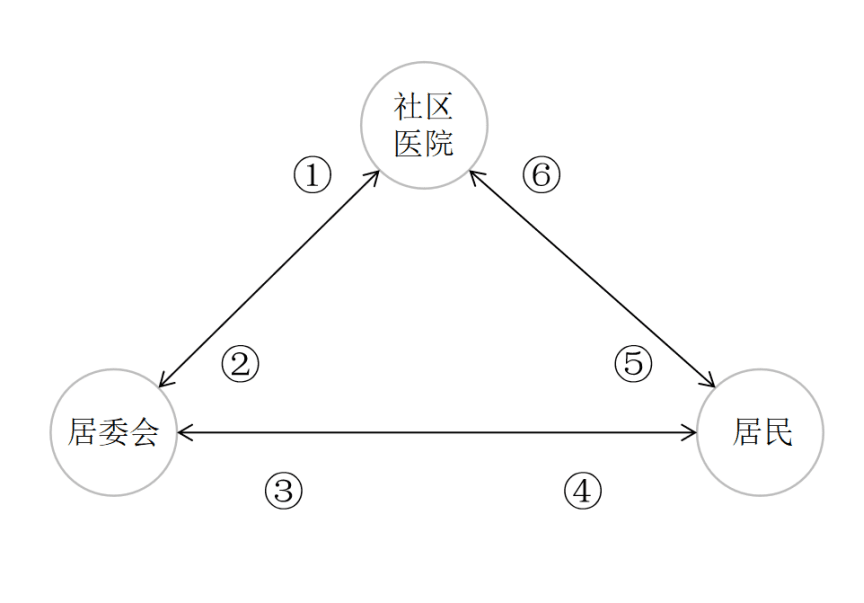
\includegraphics[scale=0.2]{guanxi.png}
    \centering
    \caption{互动关系说明}
\end{figure}
\begin{spacing}{0.9}
\begin{enumerate}
    \item ①居委会与社区医院取得联系,作为居民与社区医院的桥梁,并能将居民的诉求反馈给社区医院
    \item 社区医院为居委会提供专业人员和专业知识
    \item 居民向居委会反馈基层卫生情况,并向居委会反映医疗诉求
    \item 居委会为居民的医疗保健活动提供场地,组织居民参与到活动中来,并对居民进行随访
    \item 社区医院为居民提供专业的医疗服务,传播“治未病”知识
    \item 居民为社区医院提供病案的真实反馈
\end{enumerate}
\end{spacing}